






\subsubsection{Calcul des longueurs d'ondes des raies $K_{\alpha}$ et $K_{\beta}$ émis par le molybdène}


Tout d'abord, en utilisant le tableau \ref{tab: Tableau des nergies de niveaux lectroniques du Molybdne et du Zirconium}, nous pouvons déduire l'énergie du photon émis par la transition électronique $\Delta E(eV)$. 

\begin{table}[h!]
	\centering
	\begin{tabular}{|l|c|c|c|c|}
		\hline
		\textbf{Énergie des niveaux électroniques (keV)} & K     & $L_{\mathrm{III}}$ &$L_{\mathrm{II}}$ & $M_{\mathrm{III}}$ \\ \hline
		Molybdène      (Mo)                                  & 20.03 & 2.56 & 2.66 & 0.42 \\ \hline
		Zirconium      (Zn)                                  & 18.02 &      &      &      \\ \hline
	\end{tabular}
	\caption{Énergies des niveaux électroniques du molybdène et du zirconium}
	\label{tab: Tableau des nergies de niveaux lectroniques du Molybdne et du Zirconium}
\end{table}


Exemple pour la transition électronique $L_{\mathrm{III}} \to K$ pour le molybdène, on a : 
\vspace{0.2cm}
\begin{equation*}	
	\begin{split}
		\Delta E  & = E(K) - E(L_{\mathrm{III}})  \\
		& = 20.06 - 2.56  \\
		& = 17.47keV
	\end{split}	
\end{equation*}

Ensuite, en appliquant l'équation \ref{eq: Energie_longueur_donde}, on obtient la longueur d'onde du photon émit lors d'une transition électronique.

\begin{equation}\label{eq: Energie_longueur_donde}
	\Delta E(eV) = \frac{1.24}{\lambda (\mu m)}
\end{equation}

\newpage
Et enfin, on réalise le tableau \ref{tab: Transition nergitique en les diffrentes couche du molybdne et les diffrentes longueurs donde misse par les transitions}. 
\begin{table}[h!]
	\centering
	\begin{tabular}{|c|c|c|}
		\hline
		\multicolumn{1}{|l|}{\textbf{Transition}} & \multicolumn{1}{l|}{\textbf{Energie (keV)}} & \multicolumn{1}{l|}{\textbf{Longueur d'onde}} \\ \hline
		$L_{\mathrm{III}} \to K \ (K_{\alpha_1}) $                    & 17.47                                       & 0.709 \AA                                       \\ \hline
		$L_{\mathrm{II}} \to K \ (K_{\alpha_2}) $                      & 17.37                                       & 0.713 \AA                                       \\ \hline
		$M_{\mathrm{III}} \to K \ (K_{\beta}) $                         & 19.61                                       & 0.632 \AA                                       \\ \hline
	\end{tabular}
	\caption{\centering Longueurs d'ondes des rayons X émis par le molybdène lors des transitions électroniques $K_{\alpha}$ et $K_{\beta}$}
	\label{tab: Transition nergitique en les diffrentes couche du molybdne et les diffrentes longueurs donde misse par les transitions}
\end{table}





\subsubsection{Mesure de l’intensité ($I$) en fonction de l’angle ($\theta$)}
Dans cette partie, nous allons analyser le plan (200) un monocristal de NaCl à l'aide d'un système de diffraction des rayons X (figure \ref{fig:machine-diffraction-rx})

\begin{figure}[h!]
	\centering
	\includegraphics[width=0.7\linewidth]{"Réflexion de Bragg/Machine diffraction RX"}
	\caption{\centering Photo du système de diffraction des rayons X avec (1) : collimateur, (2) : filtre de Zn, (3) : monocristal de NaCl, (4): Compteur Geiger Muller, (5) : angle $\theta$, (6) : rayon X, (7) : plan (200) du monocristal de NaCl }
	\label{fig:machine-diffraction-rx}
\end{figure}



Pour analyser le plan (200) du monocristal NaCl, le système de diffraction des rayons X déplace le système \{tube compteur + monocristal\} d'un angle $\theta$. Pour notre analyse, nous aurons $\theta$ compris dans l'intervalle $[4^\circ, 24^\circ]$ avec un pas de $\Delta \theta = 0.1^\circ$. De plus, dans un premier temps, nous réaliserons la mesure sans le filtre au Zn, puis nous effectuerons une seconde mesure avec le filtre et commenterons les effets de ce filtre sur la réponse.












\newpage

L'objectif de cette partie est déterminer le paramètre de maille $a_0$ de la maille de NaCl représentée sur le figure \ref{fig:cristalnacl}
\begin{figure}[h!]
	\centering
	
\tdplotsetmaincoords{75}{110} % Définir les angles de vue
\begin{tikzpicture}[scale=2, tdplot_main_coords,axis/.style={->},thick]  
	
	\foreach \x in {0,1,2}
	\foreach \y in {0,1,2}
	\foreach \z in {0,1,2}
	{
		\draw[thick,opacity=1] (\x,0,\z) -- (\x,2,\z);
		\draw[thick,opacity=1] (0,\y,\z) -- (2,\y,\z);
		\draw[thick,opacity=1] (\x,\y,0) -- (\x,\y,2);
	}
	% --- labels for vertices
	\foreach \x in {0,1,2}
	\foreach \y in {0,1,2}
	\foreach \z in {0,1,2}
	{\draw[fill=gray!50] (\x,\y,\z) circle (0.3em);}    
	
	\foreach \x/\y in {1/0,2/1,1/2,0/1}
	\foreach \z in {0,2}
	{\draw[fill=orange] (\x,\y,\z) circle (0.4em);}
	
	\foreach \x/\y in {2/0,2/2,0/2,0/0}
	\foreach \z in {1}
	{\draw[fill=orange] (\x,\y,\z) circle (0.4em);}
	
	\foreach \x/\y in {1/0,2/1,1/2,0/1}
	\foreach \z in {1}
	{\draw[fill=gray!50] (\x,\y,\z) circle (0.3em);}
	
	\foreach \x/\y in {1/1}
	\foreach \z in {0,2}
	{\draw[fill=gray!50] (\x,\y,\z) circle (0.3em);}
	
	\foreach \x/\y in {1/1}
	\foreach \z in {1}
	{\draw[fill=orange] (\x,\y,\z) circle (0.4em) ;}
	
	
	\draw[thick,->, red] (2,0,0) -- (0,	0,0) node[pos=0.65,anchor=west]{\(\vec{c}\)};
	\draw[thick,->, red] (2,0,0) -- (2,2,0) node[pos=0.7, anchor=north]{\(\vec{b}\)};
	\draw[thick,->, red] (2,0,0) -- (2,0,2) node[pos=0.9, anchor=west]{\(\vec{a}\)};
	
	\draw (2, -1, 1.5) node[circle,fill=orange,scale=0.5] {} node[anchor=south west] {Cl$^-$};  
	
	\draw (2, -1, 2) node[circle,fill=gray!50,scale=0.5] {} node[anchor=south west] {Na$^+$};  
	
	\filldraw[fill=green!50!black, opacity=0.5] (2,2,1) -- (0,2,1) -- (0,0,1) -- (2,0,1) -- cycle;
	
	\draw (2.5, 3, 2) node[anchor=south west, green!50!black] {(200)};  
	
	\draw[thick,-, blue] (2,2,0) -- (2,	2,1) node[pos=0.77,anchor=west]{\(d_{200}\)};
	
	\draw[thick,-, blue] (0,2,0) -- (0,	2,2) node[pos=0.3,anchor=west]{\(a_0\)};
\end{tikzpicture}


% Dans cet exemple, j'ai utilisé pos=1.1, ce qui place le "node" juste après la fin du vecteur (à 110% du chemin, pour ainsi dire). L'anchor=west signifie que le côté ouest (gauche) du "node" est aligné avec ce point.  %
	\caption{\centering Maille de NaCl de paramètre de maille $a_0$, $\left(\vec{a}, \vec{b}, \vec{c}\right)$ : base directe du réseau réel de la maille de NaCl.}
	\label{fig:cristalnacl}
\end{figure}







Après avoir lancé l'expérience grâce au système présenté figure \ref{fig:machine-diffraction-rx}, nous obtenons la figure \ref{fig:spectre-de-diffraction-de-nacl}





\begin{figure}[h!]
	\centering
	\includegraphics[width=1\linewidth]{"Réflexion de Bragg/Spectre de diffraction de NaCl"}
	\caption{\centering Spectre en intensité du monocristal en fonction de l'angle $\beta$ équivalent à l'angle $\theta$ de la figure \ref{fig:machine-diffraction-rx}, \textbf{courbe noir} : Spectre sans le filtre Zn, {\color{red}\textbf{courbe rouge}} : Spectre avec le filtre Zn, $ .{\color{blue} \theta_1} = 6.4^\circ$ : angle de diffraction de la 1ère raie et $ {\color{blue} \theta_2}=7.2^\circ$ : angle de diffraction de la 2nd raie  }
	\label{fig:spectre-de-diffraction-de-nacl}
\end{figure}



	
\subsubsection{Interprétation de la mesure de l’intensité ($I$) en fonction de l’angle ($\theta$)}
Nous parlons de spectre en intensité avec l'intensité du rayon X incident en proportionnel aux nombre de coup par second comptabilisé par le compteur Geiger Muller présent sur la figure \ref{fig:machine-diffraction-rx}.
	
\begin{flushleft}
	\textbf{Type de transition électronique pour la première raie}	
\end{flushleft}

Dans un premier temps, nous pouvons affirmer que nous obtenons la diffraction d'angle $\theta_1$ d'un photon dû à une transition $K_{\beta}$, car la longueur d'onde émise par ce photon lors de cette transition est la plus courte par rapport à celui émis lors d'une transition $K_{\alpha_1}$ ou $K_{\alpha_2}$ d'après le tableau \ref{tab: Transition nergitique en les diffrentes couche du molybdne et les diffrentes longueurs donde misse par les transitions}.

Conformément à la loi de Bragg (équation \ref{eq:Loi_de_Bragg}) il y a nécessité d'un angle faible pour la raie $K_{\beta}$ justifie donc que la première raie observée est bien une $K_{\beta}$.

\begin{flushleft}
	\textbf{Type de transition électronique pour la seconde raie}	
\end{flushleft}

\textbf{Raisonnement par l'absurde : } supposons que la seconde raie visible soit une $K_{\beta}$. \textbf{(H)} \

\vspace{0.2cm}

Cela signifie donc que la seconde raie est d'ordre de diffraction $n=2$ correspondant avec un angle de diffraction $\theta_2$.
Ainsi, en appliquant la loi de Bragg (\ref{eq:Loi_de_Bragg}) au plan (200) pour un photon émis lors d'une transition $K_{\beta}$ de longueur d'onde $\lambda_{K_{\beta}} = 0.632 \ \AA$ (tableau \ref{tab: Transition nergitique en les diffrentes couche du molybdne et les diffrentes longueurs donde misse par les transitions}) et diffracté sous un angle $\theta_{2}$, nous avons :
\begin{equation} \label{eq: photon K_beta + Bragg}
	\frac{\lambda_{K_{\beta}}}{2d_{200}}=\frac{\sin(\theta_{2})}{2}
\end{equation}

Cependant, nous avons démontré que la première raie était dû à photon émis par une transition de type $K_{\beta}$, donc pour cette raie on a $n=1$ et un angle de diffraction $\theta_{1}$, et donc d'après la loi de Bragg (\ref{eq:Loi_de_Bragg}) :

\begin{equation} \label{eq: constant Bragg}
	\frac{\lambda_{K_{\beta}}}{2d_{200}}=\sin(\theta_{1}) = cte
\end{equation}

Par conséquent, selon (\ref{eq: constant Bragg}) et (\ref{eq: photon K_beta + Bragg}), nous obtenons :

\begin{equation}
	\frac{\sin(\theta_{2})}{2} = \sin(\theta_{1})
\end{equation}

Cependant, après calcul à l'aide de la figure \ref{fig:spectre-de-diffraction-de-nacl} :

\begin{equation} \label{eq:Inegalite_theta}
	\frac{\sin(\theta_{2})}{2} < \sin(\theta_{1})
\end{equation}

Ainsi, $(H)$ n'est pas vérifié, ce qui signifie nécessairement que nous avons une raie $K_{\alpha}$.

\newpage
Donc en appliquant périodiquement ce raisonnement nous obtenons le tableau \ref{tab:Pic_de_diffraction_et_d'interférence_du_cristal_NaCl_sur_le_plan_200}.


\begin{table}[h!]
	\centering
	\begin{tabular}{|c|c|c|c|c|}
		\hline
		$\theta$ (°) & $\sin(\theta)$ &$K_{\alpha}$ ? ou $K_{\beta}$ ? & n & $n \times \lambda $ (pm) \\ \hline
		6.4       & 0.111      & $K_{\beta}$                     & 1 & 63.2 \\ \hline
		7.2       & 0.125      &$K_{\alpha}$                    & 1 & 70.9 \\ \hline
		12.9      & 0.223      & $K_{\beta}$                     & 2  & 126.4\\ \hline
		14.5      & 0.250      &$K_{\alpha}$                    & 2  & 141.8\\ \hline
		19.6      & 0.335      & $K_{\beta}$                     & 3  & 189.6\\ \hline
		22.1      & 0.376      &$K_{\alpha}$                    & 3  & 212.7 \\ \hline
	\end{tabular}	
	\caption{Pics de diffractions et d'interférences du cristal NaCl sur le plan (200)}
	\label{tab:Pic_de_diffraction_et_d'interférence_du_cristal_NaCl_sur_le_plan_200}
\end{table}




Du tableau \ref{tab:Pic_de_diffraction_et_d'interférence_du_cristal_NaCl_sur_le_plan_200}, on trace la figure \ref{fig:courbetendance} et l'aide du programme Python (cf figure \ref{fig:photocode})


\begin{figure}[h!]
	\centering
	\includegraphics[width=1.1\linewidth]{"Réflexion de Bragg/Courbe_tendance"}
	\caption{Courbe de tendance de $n \times \lambda $(pm) et fonction de 	$\sin(\theta)$ }
	\label{fig:courbetendance}
\end{figure}


De cette courbe nous pouvons déduire le paramètre de maille $a_0$ du monocristal car d'après la figure \ref{fig:cristalnacl} on a :
	
	\begin{equation}\label{eq: paramètre de maille et d_200}
		a_0=2d_{200}
	\end{equation}

	
De plus, si on applique la loi de Bragg (équation \ref{eq:Loi_de_Bragg}) au plan $(200)$ du monocristal de NaCl, on obtient : 

\begin{equation} \label{eq:Loi_de_Bragg_NaCl_200}
	\sin (\theta ) = \frac{n \lambda }{2 d_{200}}
\end{equation}
	
	
Donc, d'après (\ref{eq: paramètre de maille et d_200}) l'équation (\ref{eq:Loi_de_Bragg_NaCl_200}) devient :
	
	\begin{equation}\label{eq: Bragg et paramètre de maille}
		n \times \lambda = a_0sin(\theta)
	\end{equation}
	
	
	Donc d'après l'équation (\ref{eq: Bragg et paramètre de maille}), $a_0$ est le coefficient directeur de la courbe  de tendance tracer sur la figure \ref{fig:courbetendance}, on en déduit donc :
	
	\begin{equation}
		\boxed{a_0 = 564.6 \ pm}
	\end{equation}
	




%%% Interprétation 
 \begin{flushleft}
	\textbf{Vérification de la valeur de $a_0$:}
\end{flushleft}



En représentant le plan (200) du monocristal de NaCl vu de dessus, nous obtenons la figure \ref{fig:Plan (200) du monocristal de NaCl vu de dessus} en supposant que le cristal respecte ses deux règles de stabilité :

\begin{itemize}
	\item Il y a un contact (ou tangence) entre les ions $Na^+$ et $Cl^-$ les plus proches voisins;
	\item Il n'existe aucun contact entre anions-anions ou cations-cations.
\end{itemize}
	



	

\begin{figure}[h!]
	\centering
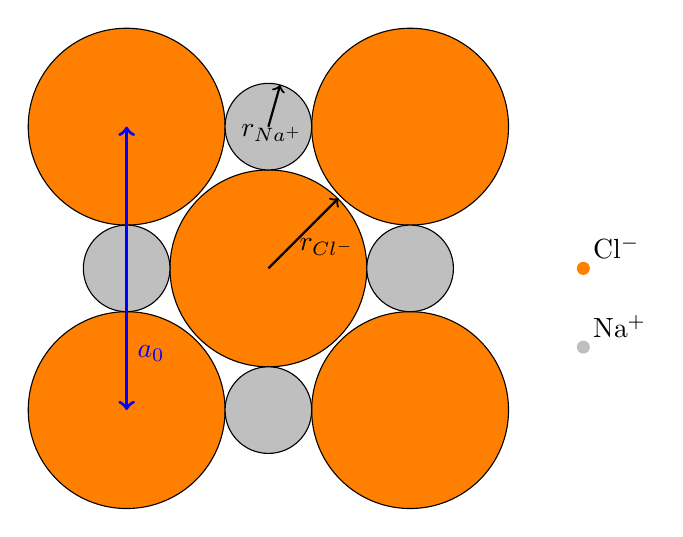
\begin{tikzpicture}
	
	
	
	% Blue Circles
	\foreach \pos in {(0,0) , (-1.8,-1.8), (1.8,1.8), (1.8,-1.8), (-1.8,1.8)} {
		\draw[fill=orange] \pos circle (1.25);
	}
	
	\foreach \pos in {(0,1.8), (0,-1.8), (-1.8,0), (1.8,0) } {
		\draw[fill=gray!50] \pos circle (0.55);
	}
	% Lines
	
	% Légende
	\draw (4, 0) node[circle,fill=orange,scale=0.5] {} node[anchor=south west] {Cl$^-$};  
	
	\draw (4, -1) node[circle,fill=gray!50,scale=0.5] {} node[anchor=south west] {Na$^+$};  
	
	\draw[thick,->, black] (0,0) -- (0.89,0.89) node[pos=0.3,anchor=west]{\(r_{Cl^-}\)};
	
	\draw[thick,->, black] (0,1.8) -- (0.15,2.33) node[pos=0.3,anchor=north]{\(r_{Na^+}\)};
	% Label
	
	\draw[very thick,<->, blue] (-1.8,-1.8) -- (-1.8,1.8) node[pos=0.2,anchor=west]{\(a_0\)};
\end{tikzpicture}
	\caption{\centering Plan (200) du monocristal de NaCl vu de dessus, $r_{Na^+}$ : rayon du cation $Na^+$, $r_{Cl^-}$ : rayon de l'anion $Cl^-$}
	\label{fig:Plan (200) du monocristal de NaCl vu de dessus}
\end{figure}

	
	D'après la figure \ref{fig:Plan (200) du monocristal de NaCl vu de dessus}, on en déduit que :
	
	\begin{equation}
		a_0 = 2r_{Na^+}+2r_{Cl^-}
	\end{equation}

avec 
\begin{itemize}
	\item $r_{Na^+}= 98 \ pm$
	\item $r_{Cl^-}= 181 \ pm $	
\end{itemize}


\vspace{0.2cm}

\begin{flushleft}
	\textbf{Application numérique :}
\end{flushleft}

	
	\begin{equation}
		a_0 = 558 \ pm
	\end{equation}
	
On a un écart de $ \pm \ 6.6\  pm$,  soit une de erreur de $1.1 \ \%$
\begin{flushleft}
	\textbf{Interprétation :}
\end{flushleft}


D'après la figure \ref{fig:courbetendance} nous obtenons une courbe de tendance de la forme :

\begin{equation}
	y=a x + b
\end{equation}
où :
\begin{itemize}
	\item $a =564.6 \ pm$ 
	\item $b = 0.4722 \ pm$
\end{itemize}
\vspace{0.2cm}
Ainsi, cela signifie que lorsque nous avons un rayon X qui arrive de manière colinéaire au plan (200) avec un angle $\theta = 0^\circ$, nous obtenons $n \times \lambda = 0.4722 \ pm$. Il en résulte qu'il existe un rayon X diffracté par le plan (200), ce qui semble incohérent. Cependant, il est possible d'admettre une certaine incertitude sur l'angle $\theta$, ce qui expliquerait pourquoi notre valeur de $b$ n'est pas nulle.



On pose :

\begin{equation}
	R = \frac{\sin(\theta_{K_{\alpha}})}{\sin(\theta_{K_{\beta}})}
\end{equation}


 \begin{flushleft}
	\textbf{Calcul du R (théorique) : $R_{th}$}
\end{flushleft}


Pour le photon émis par une transition électronique $(K_{\alpha})$ de longueur d'onde $\lambda_{K_{\alpha}}$diffracté sur le plan (200) d'un angle $\theta_{K_{\alpha}}$, on obtient la loi de Bragg (\ref{eq:Loi_de_Bragg}) suivante :

\begin{equation}\label{eq: Bragg_photon_K_alpha}
	2 d_{200}\sin(\theta_{K_{\alpha}}) = n\lambda_{K_{\alpha}}
\end{equation}

Pour le photon émis par une transition électronique $(K_{\beta})$ de longueur d'onde $\lambda_{K_{\beta}}$ diffracté sur le plan (200) d'un angle $\theta_{K_{\beta}}$, on obtient la loi de Bragg (\ref{eq:Loi_de_Bragg}) suivante :

\begin{equation}\label{eq: Bragg_photon_K_beta}
	2 d_{200}\sin(\theta_{K_{\beta}}) = n\lambda_{K_{\beta}}
\end{equation}

Donc d'après (\ref{eq: Bragg_photon_K_alpha}) et \ref{eq: Bragg_photon_K_beta} on a :
\begin{equation}\label{eq:R_{th}}
	R_{th} = \frac{\lambda_{K_{\alpha}}}{\lambda_{K_{\beta}}} 
\end{equation}


 \begin{flushleft}
	\textbf{Application numérique :}
\end{flushleft}


D'après le tableau \ref{tab: Transition nergitique en les diffrentes couche du molybdne et les diffrentes longueurs donde misse par les transitions} on a :

\begin{equation}\label{eq:A.N lambda}
	\lambda_{K_{\alpha}} = \frac{0.713 + 0.709}{2} = 0.711 \ \AA, \ \lambda_{K_{\beta}} =0.632 \ \AA
\end{equation}

Donc d'après (\ref{eq:R_{th}}) et (\ref{eq:A.N lambda}) on a :  
\begin{equation}\label{eq:R_{th}_A.N}
	R_{th} = 1.125
\end{equation}

\newpage
Ensuite, on calcule la valeur de R mesurée par l'expérience pour chaque ordre de diffraction n en utilisant le tableau \ref{tab:Pic_de_diffraction_et_d'interférence_du_cristal_NaCl_sur_le_plan_200}, puis on les compare à la valeur de $R_{th}$ dans le tableau \ref{tab:R en fonction de n}.





	
	
	
	



\begin{table}[h!]
	\centering
	\begin{tabular}{|c|c|c|}
		\hline
		$R_{th}$& $R$ (mesurée) & $n$ \\ \hline
		1.125 &1.126 & 1 \\ \hline
		1.125 &1.121& 2 \\ \hline
		1.125 & 1.122& 3 \\ \hline
	\end{tabular}
	\caption{R en fonction de n}
	\label{tab:R en fonction de n}
\end{table}




Nous remarquons que la valeur de $R$ (mesurée) $= R_{th}$ au chiffre des millièmes près, ce qui valide la théorie.

 \begin{flushleft}
	\textbf{Intérêt du filtre de Zn}
\end{flushleft}







 
Ensuite, l'intérêt du filtre de Zn consiste à supprimer les raies présentant la plus forte énergie. Lorsqu'un rayonnement X dû à une transition $K_{\beta}$ arrive au filtre de Zn, il possède suffisamment d'énergie pour ioniser l'atome de Zn (effet photoélectrique), entraînant ainsi sa disparition comme le synthétise la figure \ref{fig: Effet photoélectrique de le métal de Zn}. C'est pourquoi, comme on peut le voir sur la courbe rouge de la figure \ref{fig:spectre-de-diffraction-de-nacl}, les pics de $K_{\beta}$ sont fortement atténués, favorisant ainsi le pic de $K_{\alpha}$. 

\begin{figure}[h!]
	\centering
	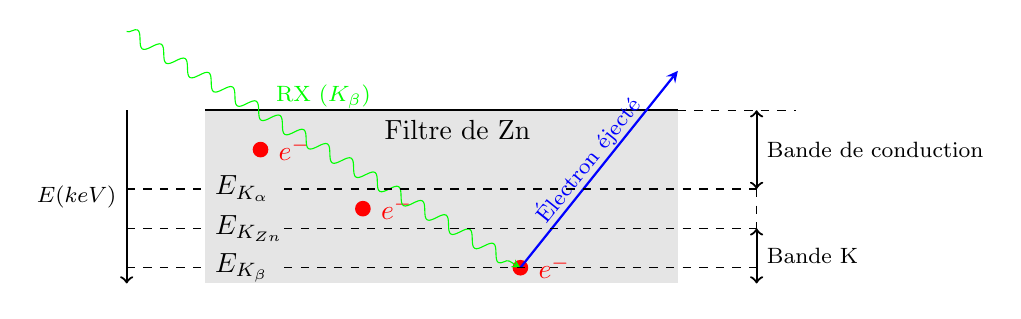
\begin{tikzpicture}[photon/.style={-stealth,decorate,decoration={snake,post length=1mm}}]
	
	% Dessiner le métal
	\fill[gray!20] (0,0) rectangle ++(6,-2.2);
	\draw[thick] (0,0) -- ++(6,0);
	\node[anchor=north] at (3.2,0) {Filtre de Zn};
	
	% Dessiner les électrons dans le métal
	\foreach \x/\y in {0.7/-0.5,2/-1.25,4/-2/-0.5}{
		\draw (\x,\y) node[circle,fill,inner sep=2pt, color=red,label={east:${\color{red}e^-}$}] {}; 
	}
	
	% Dessiner le photon incident
	\draw[photon,green] (-1,1) -- node[above=4mm,font=\footnotesize] {RX $(K_{\beta})$} ((4,-2);
	
	% Dessiner l'électron éjecté
	\draw[-stealth,blue,thick] (4,-2) -- node[above=-1mm,font=\footnotesize, sloped] {Électron éjecté} ++(2,2.5);
	
	
	\draw[<->, thick] (7,0) -- node[midway, right,font=\footnotesize] {Bande de conduction} (7,-1);
	
	\draw[dashed] (6,0) -- (7.5,0);
	
	\draw[dashed] (7,-1) -- (7,-1.5);
	
	\draw[<->, thick] (7,-1.5) -- node[midway, right,font=\footnotesize] {Bande K} (7,-2.2);
	
	\draw[->, thick] (-1,0) -- node[midway, left,font=\footnotesize] {$E(keV)$} (-1,-2.2);
	
	\foreach \y/\x  in {-1/$E_{K_{\alpha}}$, -1.5/$E_{K_{Zn}}$, -2/$E_{K_{\beta}}$} 
	{
		\draw [dashed] (-1,\y) -- (0,\y) node[right] {\x};
		\draw[dashed] (1,\y) -- (7,\y);
	}
	

	
\end{tikzpicture}



	\caption{\centering Effet photoélectrique dans le filtre de Zn , $E_{K_{\alpha}}$ : énergie d'une transition $K_{\alpha}$, $E_{K_{\beta}}$ : énergie d'une transition $K_{\beta}$, $E_{K_{Zn}}$ : niveau d'énergie de la bande K du cristal de Zn avec l'ensemble des énergies sont répertoriés dans les tableaux \ref{tab: Tableau des nergies de niveaux lectroniques du Molybdne et du Zirconium} et \ref{tab: Transition nergitique en les diffrentes couche du molybdne et les diffrentes longueurs donde misse par les transitions}}
	\label{fig: Effet photoélectrique de le métal de Zn}
\end{figure}


De plus, dans le cas d'une analyse plus complexe de plusieurs plans du cristal, cela nous permet de réduire la quantité d'informations reçues par le logiciel, ce qui facilite l'interprétation de la courbe obtenue. Sans le filtre, l'information utile serait répétée deux fois.






